\chapter{Hückeltheorie en geconjugeerde systemen}\label{ch:b2:huckel}

Voeg waterstof toe aan cyclohexeen en er komt per mol \qty{119}{kJ} vrij. Benzeen,
met drie dubbele bindingen in een ring van zes koolstofatomen, zou op weg naar cyclohexaan driemaal
zoveel moeten vrijgeven; het geeft \qty{150}{kJ} minder vrij. Die ontbrekende
energie is de stabiliteit van een \omterm{def:b2:huckel:aromatic}{aromatische} ring, de reden waarom benzeen weerstand biedt aan
de addities die alkenen ondergaan. In 1931 berekende Erich Hückel haar met een
determinant, na het molecuul herleid te hebben tot zijn $\pi$-elektronen en hun
buren. Zijn methode is ruw, maar ze verklaart waarom ringen met zes $\pi$-elektronen
bijzonder zijn, waarom lange geconjugeerde ketens zichtbaar licht absorberen, en
waar een geconjugeerd molecuul zijn ladingen draagt.

\begin{recall}
\Cref{ch:b2:diatomic-mos}: \omterm{def:b2:diatomic-mos:integrals}{coulombintegraal} $\alpha$, \omterm{def:b2:diatomic-mos:integrals}{resonantie-integraal} $\beta$,
\omterm{def:b2:diatomic-mos:integrals}{seculiere determinant}. \Cref{ch:b2:fragment-orbitals}: $\pi$-orbitalen van etheen en
allyl. Het deel van jaar~1: geconjugeerde systemen, resonantie, chromoforen en
absorptiemaxima.
\end{recall}

\section{De hückelmethode}

In een vlak geconjugeerd molecuul zijn de $\sigma$-orbitalen symmetrisch en de p-orbitalen
loodrecht op het vlak antisymmetrisch ten opzichte van dat vlak: ze
mengen niet (\cref{prop:b2:diatomic-mos:symmetry}), en de $\pi$-elektronen kunnen
apart behandeld worden.

\begin{definition}[Hückelmethode]\label{def:b2:huckel:method}
De \emph{hückelmethode}\index{huckelmethode@hückelmethode} berekent de $\pi$-orbitalen van een
vlak geconjugeerd systeem als combinaties $\psi = \sum_r c_r p_r$ van één p-orbitaal per
atoom, met de benaderingen: overlappen $S_{rs} = 0$ voor $r \neq s$ (en 1 voor $r =
s$); \omterm{def:b2:diatomic-mos:integrals}{coulombintegralen} allemaal gelijk aan $\alpha$; \omterm{def:b2:diatomic-mos:integrals}{resonantie-integralen} gelijk aan $\beta < 0$
tussen gebonden buren en anders nul.
\end{definition}

Met $x = (\alpha - E)/\beta$ worden de seculiere vergelijkingen, voor elk atoom $r$,
$xc_r + \sum_{s \text{ gebonden aan } r} c_s = 0$, en de energieën zijn de wortels van een
determinant met $x$ op de diagonaal en 1 tussen gebonden atomen. Gelijkwaardig is $E =
\alpha + m\beta$, waarin de $m$ de eigenwaarden zijn van de nabuurmatrix van het
koolstofskelet van het molecuul; omdat $\beta < 0$, is een positieve $m$ een bindend niveau.

\begin{method}[Een hückelberekening]\label{met:b2:huckel:huckel}
\begin{enumerate}
  \item Nummer de geconjugeerde atomen; schrijf de matrix met 0 op de diagonaal en 1
        voor elk gebonden paar.
  \item Bepaal haar eigenwaarden $m_k$ (met de gesloten vormen hieronder, of numeriek): $E_k =
        \alpha + m_k\beta$.
  \item Vul de niveaus vanaf het meest bindende, twee elektronen per niveau:
        $E_\pi = \sum_k n_k E_k$.
  \item Bereken uit de genormeerde coëfficiënten de ladingen en de bindingsindices.
\end{enumerate}
\end{method}

\begin{proposition}[Spoor]\label{prop:b2:huckel:trace}
De energieën van de $n$ $\pi$-orbitalen van een hückelsysteem tellen op tot $n\alpha$.
\end{proposition}

\begin{proof}
De som van de eigenwaarden van een matrix is haar spoor; de hückelmatrix heeft $\alpha$
op elk van haar $n$ diagonaalelementen.
\end{proof}

\section{Lineaire polyenen}

\begin{theorem}[Niveaus van een lineaire keten]\label{thm:b2:huckel:polyene}
Een lineaire geconjugeerde keten van $n$ atomen heeft de niveaus en coëfficiënten
\[
  E_k = \alpha + 2\beta\cos\frac{k\pi}{n + 1}, \qquad
  c_{jk} = \sqrt{\frac{2}{n + 1}}\,\sin\frac{jk\pi}{n + 1}, \qquad k = 1, \dots, n .
\]
\end{theorem}

\begin{proof}
De seculiere vergelijkingen zijn $c_{j-1} + xc_j + c_{j+1} = 0$ voor $j = 1, \dots, n$, met
$c_0 = c_{n+1} = 0$. Probeer $c_j = \sin j\theta$: $\sin(j - 1)\theta + \sin(j + 1)\theta = 2\sin
j\theta\cos\theta$, dus de vergelijkingen gelden met $x = -2\cos\theta$, en $c_0 = 0$
automatisch. De randvoorwaarde $c_{n+1} = \sin(n + 1)\theta = 0$ geeft $\theta =
k\pi/(n + 1)$. Dan is $E = \alpha - x\beta = \alpha + 2\beta\cos\theta$. De normering gebruikt
$\sum_{j=1}^n\sin^2 j\theta = (n + 1)/2$.
\end{proof}

\begin{example}[Butadieen]\label{ex:b2:huckel:butadiene}
Voor $n = 4$: $E = \alpha \pm 1.618\beta$, $\alpha \pm 0.618\beta$. Vier $\pi$-elektronen vullen de twee
bindende niveaus: $E_\pi = 4\alpha + 2(1.618 + 0.618)\beta = 4\alpha + 4.472\beta$. De laagste
orbitaal heeft coëfficiënten 0.372, 0.602, 0.602, 0.372, de volgende 0.602, 0.372,
$-0.372$, $-0.602$.
\end{example}

\begin{omfigure}
\begin{tikzpicture}[font=\small]
  \foreach \k/\a/\b/\c/\d/\lab in {1/0.372/0.602/0.602/0.372/{$\psi_1$, $\alpha + 1.618\beta$},
      2/0.602/0.372/-0.372/-0.602/{$\psi_2$, $\alpha + 0.618\beta$},
      3/0.602/-0.372/-0.372/0.602/{$\psi_3$, $\alpha - 0.618\beta$},
      4/0.372/-0.602/0.602/-0.372/{$\psi_4$, $\alpha - 1.618\beta$}} {
    \begin{scope}[yshift={(\k-1)*2.1cm}]
      \draw[black!40] (-0.2,0) -- (3.2,0);
      \pic at (0,0) {omp={1.6*\a}{90}}; \pic at (1,0) {omp={1.6*\b}{90}};
      \pic at (2,0) {omp={1.6*\c}{90}}; \pic at (3,0) {omp={1.6*\d}{90}};
      \node[anchor=west] at (3.6,0) {\lab};
    \end{scope}
  }
\end{tikzpicture}

{\small De vier $\pi$-orbitalen van butadieen, met lobben getekend in verhouding tot de
(berekende) hückelcoëfficiënten en gekleurd naar hun teken; de energieën stijgen
naar boven, met $0, 1, 2, 3$ knopen. De twee laagste orbitalen zijn gevuld.}
\end{omfigure}

\begin{definition}[$\pi$-ladingen en bindingsindices]\label{def:b2:huckel:indices}
Met $n_k$ elektronen in orbitaal $k$ (0, 1 of 2) en reële coëfficiënten $c_{rk}$ is de
\emph{$\pi$-lading}\index{pi-lading@$\pi$-lading} op atoom $r$ gelijk aan $q_r = \sum_k n_kc_{rk}^2$ (het
aantal $\pi$-elektronen dat het draagt), en de \emph{$\pi$-bindingsindex}\index{pi-bindingsindex@$\pi$-bindingsindex}
van de binding $rs$ gelijk aan $p_{rs} = \sum_k n_kc_{rk}c_{sk}$.
\end{definition}

Voor butadieen is $p_{12} = 2(0.372 \times 0.602 + 0.602 \times 0.372) = 0.894$ en $p_{23} =
2(0.602^2 - 0.372^2) = 0.447$: de eindbindingen dragen het grootste deel van de $\pi$-binding en zijn
de kortste, de centrale binding heeft een gedeeltelijk dubbelbindingskarakter. Alle ladingen zijn
1.

\begin{proposition}[Alternante koolwaterstoffen]\label{prop:b2:huckel:alternant}
In een neutrale koolwaterstof waarvan de geconjugeerde atomen in twee verzamelingen gekleurd kunnen worden
zonder dat twee buren tot dezelfde verzameling behoren (geen oneven ring), is elke $\pi$-lading gelijk aan 1.
\end{proposition}

\admitted

Het resultaat (Coulson en Rushbrooke) is hierboven gecontroleerd op butadieen en op benzeen door
symmetrie; het is de reden waarom zulke koolwaterstoffen geen permanente dipool van hun
$\pi$-elektronen hebben.

\begin{definition}[Delokalisatie-energie]\label{def:b2:huckel:delocalisation}
De \emph{delokalisatie-energie}\index{delokalisatie-energie} van een geconjugeerd
systeem is het verschil tussen zijn $\pi$-energie en die van hetzelfde aantal
geïsoleerde dubbele bindingen, elk met $E_\pi = 2\alpha + 2\beta$.
\end{definition}

Voor butadieen is ze $4.472\beta - 4\beta = 0.472\beta$; voor hexatrieen $0.988\beta$.

\section{Ringen en aromaticiteit}

\begin{theorem}[Niveaus van een ring]\label{thm:b2:huckel:ring}
Een vlakke ring van $n$ geconjugeerde atomen heeft de niveaus $E_k = \alpha + 2\beta\cos(2\pi k/n)$,
$k = 0, 1, \dots, n - 1$: één laagste niveau $\alpha + 2\beta$, daarna paren ontaarde
niveaus, en voor even $n$ één hoogste niveau $\alpha - 2\beta$.
\end{theorem}

\begin{proof}
In een ring heeft elk atoom twee buren, met indices modulo $n$:
$c_{j-1} + xc_j + c_{j+1} = 0$ voor alle $j$ en $c_{j+n} = c_j$. Probeer $c_j = \mathrm e^{\mathrm
i jq}$: de vergelijking geeft $x = -(\mathrm e^{-\mathrm iq} + \mathrm e^{\mathrm iq}) = -2\cos q$,
en de periodiciteit vereist $nq = 2\pi k$. De niveaus $k$ en $n - k$ hebben dezelfde
energie; hun som en verschil zijn reële orbitalen. Alleen $k = 0$ (en $k = n/2$ voor
even $n$) is enkelvoudig.
\end{proof}

\begin{corollary}[Cirkel van Frost]\label{cor:b2:huckel:frost}
De niveaus van een ring worden afgelezen op een cirkel met straal $2|\beta|$ en middelpunt $\alpha$, waarin
een regelmatige $n$-hoek is ingeschreven met één hoekpunt onderaan: elk hoekpunt ligt
op de hoogte van een niveau.
\end{corollary}

\begin{proof}
Hoekpunt $k$ staat onder de hoek $-\pi/2 + 2\pi k/n$, op hoogte
$-2|\beta|\cos(2\pi k/n) = 2\beta\cos(2\pi k/n)$ ten opzichte van het middelpunt.
\end{proof}

\begin{omfigure}
\begin{tikzpicture}[font=\scriptsize]
  \foreach \n/\x/\name/\el in {4/0/{\ce{C4H4}}/4, 5/3.4/{\ce{C5H5-}}/6, 6/6.8/{\ce{C6H6}}/6, 7/10.2/{\ce{C7H7+}}/6} {
    \begin{scope}[xshift=\x cm]
      \draw[black!35] (0,0) circle (1.2);
      \draw[black!60] \foreach \k in {0,...,\the\numexpr\n-1\relax} { ({-90+360*\k/\n}:1.2) -- ({-90+360*(\k+1)/\n}:1.2) };
      \foreach \k in {0,...,\the\numexpr\n-1\relax} {
        \draw[very thick] ({1.2*cos(-90+360*\k/\n)-0.22},{1.2*sin(-90+360*\k/\n)}) -- ({1.2*cos(-90+360*\k/\n)+0.22},{1.2*sin(-90+360*\k/\n)});
      }
      \draw[densely dotted] (-1.5,0) -- (1.5,0);
      \node[font=\small] at (0,-1.75) {\name};
    \end{scope}
  }
  \node[anchor=east] at (-1.5,0) {$\alpha$};
  % electrons: C4H4 (2 + 1 + 1), others filled lowest three
  \foreach \x in {0,3.4,6.8,10.2} {
    \draw[-{Stealth[length=1mm]}, thick] ({\x-0.05},-1.32) -- ({\x-0.05},-1.08);
    \draw[-{Stealth[length=1mm]}, thick] ({\x+0.05},-1.08) -- ({\x+0.05},-1.32);
  }
  % six-electron rings: the lowest degenerate pair is filled
  \foreach \n/\x in {5/3.4, 6/6.8, 7/10.2} {
    \foreach \k in {1, \the\numexpr\n-1\relax} {
      \pgfmathsetmacro\ex{\x + 1.2*cos(-90 + 360*\k/\n)}
      \pgfmathsetmacro\ey{1.2*sin(-90 + 360*\k/\n)}
      \draw[-{Stealth[length=1mm]}, thick] ({\ex-0.05},{\ey-0.12}) -- ({\ex-0.05},{\ey+0.12});
      \draw[-{Stealth[length=1mm]}, thick] ({\ex+0.05},{\ey+0.12}) -- ({\ex+0.05},{\ey-0.12});
    }
  }
  % C4H4: one electron in each of the two nonbonding levels
  \draw[-{Stealth[length=1mm]}, thick] (1.2,-0.12) -- (1.2,0.12);
  \draw[-{Stealth[length=1mm]}, thick] (-1.2,-0.12) -- (-1.2,0.12);
\end{tikzpicture}

{\small Cirkels van Frost. De hoekpunten van elke veelhoek, ingeschreven met een hoekpunt
onderaan in een cirkel met straal $2|\beta|$, geven de niveaus van de ring. Met zes $\pi$-elektronen
vullen \ce{C5H5-}, \ce{C6H6} en \ce{C7H7+} het laagste niveau en één ontaard
paar: gesloten schillen. De vier elektronen van cyclobutadieen laten twee elektronen achter in een
ontaard niet-bindend paar (getekend).}
\end{omfigure}

\begin{definition}[Aromaticiteit]\label{def:b2:huckel:aromatic}
Een cyclisch, vlak, volledig geconjugeerd systeem is \emph{aromatisch}\index{aromatisch} wanneer
zijn $\pi$-elektronen een gesloten schil vormen met een grote \omterm{def:b2:huckel:delocalisation}{delokalisatie-energie}, en
\emph{antiaromatisch}\index{antiaromatisch} wanneer zijn $\pi$-elektronen een ontaard paar half vullen,
wat het minder stabiel maakt dan de overeenkomstige open keten.
\end{definition}

\begin{theorem}[Regel van Hückel]\label{thm:b2:huckel:huckel-rule}
Een vlak monocyclisch geconjugeerd systeem heeft een gesloten schil van $\pi$-elektronen dan en slechts dan
als het er $4N + 2$ bevat ($N = 0, 1, 2, \dots$); met $4N$ heeft het twee elektronen in een
half gevuld ontaard paar. Dit is de \emph{regel van Hückel}\index{regel van Huckel@regel van Hückel}.
\end{theorem}

\begin{proof}
Volgens \cref{thm:b2:huckel:ring} zijn de niveaus vanaf onderen één enkelvoudig niveau en
daarna ontaarde paren (voor het bezette deel). Een gesloten schil vult het enkelvoudige
niveau (2 elektronen) en een geheel aantal $N$ paren (elk 4 elektronen): $4N + 2$. Met
$4N$ elektronen bevat het laatste paar er maar twee, één in elk van zijn orbitalen (regel van
Hund).
\end{proof}

\begin{method}[Is het aromatisch?]\label{met:b2:huckel:aromaticity}
\begin{enumerate}
  \item Is het systeem een ring met een p-orbitaal op elk atoom (carbokation- en
        carbanioncentra en vrije elektronenparen van heteroatomen meegerekend)?
  \item Kan het vlak zijn?
  \item Tel de $\pi$-elektronen: $4N + 2$ \omterm{def:b2:huckel:aromatic}{aromatisch}, $4N$ \omterm{def:b2:huckel:aromatic}{antiaromatisch} als het vlak is.
  \item Een \omterm{def:b2:huckel:aromatic}{antiaromatische} ring vermijdt vlakheid of conjugatie wanneer dat kan
        (cyclo-octatetraeen is kuipvormig en gedraagt zich als een polyeen).
\end{enumerate}
\end{method}

\begin{example}[Benzeen]\label{ex:b2:huckel:benzene}
Zes $\pi$-elektronen vullen $\alpha + 2\beta$ en het paar $\alpha + \beta$: $E_\pi = 6\alpha + 8\beta$.
Drie geïsoleerde dubbele bindingen geven $6\alpha + 6\beta$: de \omterm{def:b2:huckel:delocalisation}{delokalisatie-energie} is $2\beta$,
ongeveer het dubbele van die van de open keten van zes koolstofatomen, hexatrieen ($0.988\beta$): het sluiten van
de ring is evenveel waard. Door symmetrie zijn alle bindingsindices gelijk ($p = 2/3$), en ook de zes
bindingslengten, \qty{139.7}{pm}, tussen die van etheen (\qty{133.9}{pm}) en ethaan
(\qty{153.6}{pm}).
% ledger: geo:C6H6.rCC, geo:C2H4.rCC, geo:C2H6.rCC
\end{example}

\begin{omfigure}
\begin{tikzpicture}[font=\small, y=0.013cm, x=1.0cm]
  \draw[thick] (0,0) -- (10.5,0);
  \node[anchor=north] at (5.2,-8) {cyclohexaan (referentie $\Delta_r H = 0$)};
  % cyclohexene
  \draw[thick, omDef] (0.6,118.8) -- (1.6,118.8); \draw[->, omDef] (1.1,118.8) -- (1.1,4);
  \node[font=\scriptsize, anchor=south, align=center] at (1.1,120) {cyclohexeen\\ \qty{118.8}{kJ/mol}};
  % diene
  \draw[thick, omDef] (3.6,227.7) -- (4.6,227.7); \draw[->, omDef] (4.1,227.7) -- (4.1,4);
  \draw[thick, black!45, densely dashed] (4.7,237.6) -- (5.6,237.6);
  \node[font=\scriptsize, anchor=south, black!60] at (5.15,240) {$2 \times 118.8$};
  \node[font=\scriptsize, anchor=east, align=right] at (3.5,227.7) {cyclohexa-1,3-dieen\\ \qty{227.7}{kJ/mol}};
  % benzene
  \draw[thick, omDef] (7.6,206.0) -- (8.6,206.0); \draw[->, omDef] (8.1,206.0) -- (8.1,4);
  \node[font=\scriptsize, anchor=east, align=right] at (7.5,206.0) {benzeen\\ \qty{206.0}{kJ/mol}};
  \draw[thick, black!45, densely dashed] (7.6,356.4) -- (8.6,356.4);
  \node[font=\scriptsize, anchor=south, black!60] at (8.1,358) {$3 \times 118.8 = 356.4$};
  \draw[<->, omThm, thick] (8.9,206) -- (8.9,356.4) node[midway, right, font=\scriptsize] {\qty{150}{kJ/mol}};
\end{tikzpicture}

{\small Hydrogeneringsenthalpieën tot cyclohexaan in de gasfase, uit getabelleerde
vormingsenthalpieën (staven, hoogte = vrijgekomen warmte). Twee geconjugeerde dubbele bindingen
geven \qty{10}{kJ/mol} minder vrij dan tweemaal één; benzeen geeft \qty{150}{kJ/mol} minder vrij dan
driemaal één: zijn \omterm{def:b2:huckel:aromatic}{aromatische} stabilisatie.}
% ledger: dfh:C6H6_g, dfh:C6H10_g, dfh:C6H12_g, dfh:C6H8_g
\end{omfigure}

\begin{history}[De ring van Kekulé]
\begin{minipage}[t]{0.22\linewidth}
\vspace{0pt}
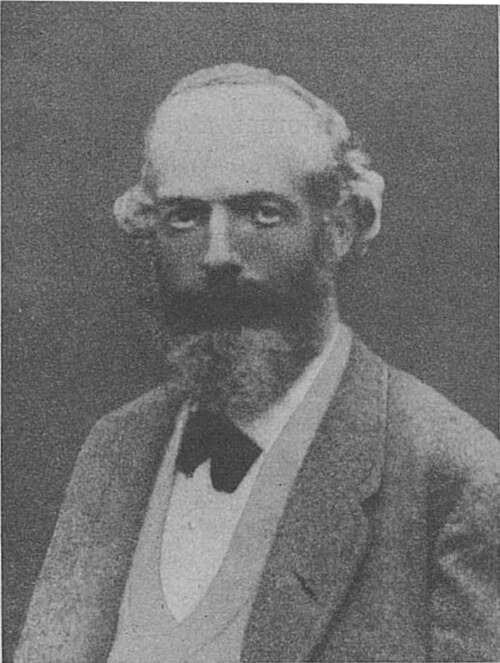
\includegraphics[width=\linewidth]{images/book3/kekule.jpg}
\end{minipage}\hfill
\begin{minipage}[t]{0.74\linewidth}
\vspace{0pt}
In 1865 stelde August Kekulé voor dat de zes koolstofatomen van benzeen een ring vormen
met afwisselend enkelvoudige en dubbele bindingen, en kort daarna dat de twee afwisselingen
zo snel uitwisselen dat elke binding dezelfde is. De gelijke bindingen die door röntgendiffractie
gevonden werden, en de $\pi$-orbitalen die over de hele ring uitgespreid zijn, gaven zijn intuïtie haar
moderne vorm; de \omterm{thm:b2:huckel:huckel-rule}{regel van Hückel} verklaarde in 1931 waarom zes elektronen, en niet vier of
acht, een ring bijzonder maken. (Portret, 1873, onbekende auteur, publiek domein,
Wikimedia Commons.)
\end{minipage}
\end{history}

\section{Conjugatie en licht}

\begin{proposition}[De kloof van een polyeen]\label{prop:b2:huckel:gap}
In een lineair polyeen van $n$ koolstofatomen ($n$ even) is de kloof tussen het hoogste bezette
en het laagste lege $\pi$-niveau gelijk aan $4|\beta|\sin(\pi/(2(n + 1)))$: ze neemt af naarmate de
keten langer wordt.
\end{proposition}

\begin{proof}
Het hoogste bezette niveau is $k = n/2$, het laagste lege $k = n/2 + 1$. Met $\theta_k =
k\pi/(n + 1)$ is $E_{n/2+1} - E_{n/2} = 2|\beta|(\cos\theta_{n/2} - \cos\theta_{n/2+1}) = 4|\beta|
\sin\frac{\theta_{n/2} + \theta_{n/2+1}}{2}\sin\frac{\theta_{n/2+1} - \theta_{n/2}}{2}$, en de
eerste sinus is $\sin(\pi/2) = 1$. Ze neemt af met $n$, omdat $\sin$ stijgend is op
$[0, \pi/2]$.
\end{proof}

\begin{omfigure}
\begin{tikzpicture}
\begin{axis}[width=0.5\linewidth, height=5cm, xmin=0, xmax=22, ymin=0, ymax=2.2,
  axis x line=bottom, axis y line=left, xlabel={koolstofatomen $n$}, ylabel={kloof$/|\beta|$},
  tick label style={font=\small}, label style={font=\small}]
\addplot[omThm, thick, mark=*, mark size=1.3pt] table[x=n, y=gap] {figdata/out/bachelor-2-huckel-b.dat};
\end{axis}
\end{tikzpicture}\hfill
\begin{tikzpicture}
\begin{axis}[width=0.48\linewidth, height=5.4cm, xmin=-1, xmax=11, ymin=-2.4, ymax=2.4,
  axis x line=none, axis y line=left, ylabel={$(E - \alpha)/|\beta|$}, clip=false,
  tick label style={font=\small}, label style={font=\small}]
\addplot[only marks, mark=-, mark size=5pt, very thick, omDef] table[x=x, y=e] {figdata/out/bachelor-2-huckel-a.dat};
\draw[densely dotted] (axis cs:-1,0) -- (axis cs:11,0);
\node[anchor=north, font=\scriptsize] at (axis cs:0,-2.45) {C$_2$};
\node[anchor=north, font=\scriptsize] at (axis cs:2,-2.45) {C$_3$};
\node[anchor=north, font=\scriptsize] at (axis cs:4,-2.45) {C$_4$};
\node[anchor=north, font=\scriptsize] at (axis cs:6,-2.45) {C$_6$};
\node[anchor=north, font=\scriptsize] at (axis cs:8,-2.45) {ring 4};
\node[anchor=north, font=\scriptsize] at (axis cs:10,-2.45) {ring 6};
\end{axis}
\end{tikzpicture}

{\small Links: de hückelkloof van lineaire polyenen daalt naarmate de keten groeit, de
reden waarom lange geconjugeerde ketens bij langere golflengten absorberen, tot in het zichtbare.
Rechts: berekende niveaus van etheen, allyl, butadieen, hexatrieen (ketens) en van
cyclobutadieen en benzeen (ringen); bindende niveaus onder $\alpha$.}
\end{omfigure}

Een heteroatoom wordt ingebracht door zijn \omterm{def:b2:diatomic-mos:integrals}{coulombintegraal} te veranderen, $\alpha_X = \alpha + h\beta$, en de
\omterm{def:b2:diatomic-mos:integrals}{resonantie-integralen} van zijn bindingen: een model met instelbare parameters, dat de
kwalitatieve resultaten behoudt (een elektronegatief atoom, $h > 0$, trekt de $\pi$-dichtheid naar
zich toe) maar waarvan de getallen aangepast zijn, niet afgeleid.

\section{Oefeningen}

\begin{exercise}[$\star$]\label{exo:b2:huckel:1}
Geef $E_\pi$ voor het allylkation, -radicaal en -anion.
\end{exercise}

\begin{exercise}[$\star$]\label{exo:b2:huckel:2}
Bereken $E_\pi$ van butadieen uit de niveaus $\alpha \pm 1.618\beta$, $\alpha \pm 0.618\beta$.
\end{exercise}

\begin{exercise}[$\star$]\label{exo:b2:huckel:3}
\omterm{def:b2:huckel:aromatic}{Aromatisch}, \omterm{def:b2:huckel:aromatic}{antiaromatisch} of geen van beide (als het vlak is): benzeen, cyclopentadienylanion,
cyclopentadienylkation, tropyliumkation \ce{C7H7+}, cyclobutadieen, vlak
cyclo-octatetraeen.
\end{exercise}

\begin{exercise}[$\star$]\label{exo:b2:huckel:4}
Teken de cirkel van Frost voor vlak cyclo-octatetraeen en plaats zijn acht $\pi$-elektronen.
\end{exercise}

\begin{exercise}[$\star\star$]\label{exo:b2:huckel:5}
Bereken de \omterm{def:b2:huckel:delocalisation}{delokalisatie-energie} van butadieen en geef ze in \unit{kJ/mol} met
$|\beta| = \qty{75}{kJ/mol}$. Vergelijk met de \qty{10}{kJ/mol} van de hydrogeneringsgegevens
voor cyclohexa-1,3-dieen.
\end{exercise}

\begin{exercise}[$\star\star$]\label{exo:b2:huckel:6}
Bereken de $\pi$-bindingsindices van butadieen en voorspel welke van zijn C--C-bindingen de
kortste is.
\end{exercise}

\begin{exercise}[$\star\star$]\label{exo:b2:huckel:7}
De niveaus van een vijfring zijn $\alpha + 2\beta$, $\alpha + 0.618\beta$ (tweemaal),
$\alpha - 1.618\beta$ (tweemaal). Vul ze voor het cyclopentadienylanion en -kation en
vergelijk.
\end{exercise}

\begin{exercise}[$\star\star$]\label{exo:b2:huckel:8}
Leg met de niveaus van een zevenring uit waarom cycloheptatrienylbromide
zich gedraagt als een zout, tropyliumbromide.
\end{exercise}

\begin{exercise}[$\star\star$]\label{exo:b2:huckel:9}
Controleer de spoorregel op hexatrieen, waarvan de niveaus $\alpha \pm 1.802\beta$, $\alpha \pm
1.247\beta$, $\alpha \pm 0.445\beta$ zijn.
\end{exercise}

\begin{exercise}[$\star\star\star$]\label{exo:b2:huckel:10}
Leid de niveaus van hexatrieen af uit de gesloten vorm, en zijn \omterm{def:b2:huckel:delocalisation}{delokalisatie-energie}.
\end{exercise}

\begin{exercise}[$\star\star\star$]\label{exo:b2:huckel:11}
Vierkant cyclobutadieen zou twee ongepaarde elektronen hebben. Leg uit waarom het echte molecuul
rechthoekig is, met twee korte en twee lange bindingen.
\end{exercise}

\begin{exercise}[$\star\star\star$]\label{exo:b2:huckel:12}
Bepaal in een $\pi$-systeem van twee atomen \ce{C=X} met $\alpha_X = \alpha + \beta$ (modelwaarde, $h = 1$) en
$\beta_{\ce{CX}} = \beta$ de twee niveaus en de $\pi$-ladingen op C en X voor twee
elektronen.
\end{exercise}

\section{Probleem: de ontbrekende energie van benzeen}

\begin{problem}[{Weekendprobleem --- de aromatische stabilisatie van benzeen uit
hydrogeneringsenthalpieën, de hückelniveaus van benzeen en zijn delokalisatie-energie,
de waarde van $|\beta|$, en de vergelijking met hexatrieen en
cyclo-octatetraeen}]
\label{pb:b2:huckel:1}
Gegevens: vormingsenthalpieën van de gassen (\unit{kJ/mol}): benzeen 82.9,
cyclohexa-1,3-dieen 104.6, cyclohexeen $-4.3$, cyclohexaan $-123.1$. Bindingslengten
(pm): benzeen 139.7, etheen 133.9, ethaan 153.6.
% ledger: dfh:C6H6_g, dfh:C6H8_g, dfh:C6H10_g, dfh:C6H12_g, geo:C6H6.rCC, geo:C2H4.rCC, geo:C2H6.rCC

\medskip
\noindent\textbf{Deel I --- Hydrogenering.}
\begin{enumerate}
  \item Bereken $\Delta_r H^\circ$ van de hydrogenering van cyclohexeen tot cyclohexaan.
  \item Hetzelfde voor cyclohexa-1,3-dieen.
  \item Hetzelfde voor benzeen.
  \item Hoeveel zouden drie onafhankelijke dubbele bindingen vrijgeven?
  \item Leid de stabilisatie van benzeen af.
  \item Vergelijk met die van het geconjugeerde dieen, en becommentarieer.
\end{enumerate}

\medskip
\noindent\textbf{Deel II --- Benzeen volgens Hückel.}
\begin{enumerate}[resume]
  \item Schrijf de hückelmatrix van benzeen op.
  \item Geef zijn niveaus uit de ringformule.
  \item Vul ze met zes $\pi$-elektronen.
  \item Bereken $E_\pi$.
  \item Bereken $E_\pi$ van drie geïsoleerde dubbele bindingen.
  \item Leid de \omterm{def:b2:huckel:delocalisation}{delokalisatie-energie} af.
  \item Controleer de spoorregel.
\end{enumerate}

\medskip
\noindent\textbf{Deel III --- De waarde van $|\beta|$.}
\begin{enumerate}[resume]
  \item Stel de \omterm{def:b2:huckel:delocalisation}{delokalisatie-energie} gelijk aan de stabilisatie van Deel I en bepaal
        $|\beta|$.
  \item Voorspel met die waarde de \omterm{def:b2:huckel:delocalisation}{delokalisatie-energie} van butadieen, en vergelijk
        met Deel I.
  \item Bereken de $\pi$-bindingsindices van benzeen.
  \item Vergelijk ze met die van butadieen.
  \item Leg uit waarom de bindingslengten van benzeen gelijk zijn en waar ze liggen.
\end{enumerate}

\medskip
\noindent\textbf{Deel IV --- Andere ringen en ketens.}
\begin{enumerate}[resume]
  \item Bereken de \omterm{def:b2:huckel:delocalisation}{delokalisatie-energie} van hexatrieen en vergelijk met benzeen.
  \item Geef de niveaus van vlak cyclo-octatetraeen.
  \item Vul ze met acht elektronen: wat is er mis?
  \item Hoe ontsnapt het echte molecuul daaraan?
  \item Wat is de situatie van cyclobutadieen?
  \item Formuleer de \omterm{thm:b2:huckel:huckel-rule}{regel van Hückel}.
  \item Geef de waarde van $|\beta|$ die verkregen wordt door de \omterm{def:b2:huckel:delocalisation}{delokalisatie-energie} van benzeen
        gelijk te stellen aan zijn gemeten stabilisatie.
\end{enumerate}
\end{problem}
